\documentclass[main.tex]{subfiles}

\begin{document}
\chapter[Структура отчёта по контрольной работе]{Структура отчёта\\ по контрольной работе}\label{ch:str}

Отчёт по контрольной работе должен содержать:

\begin{enumerate}
\item титульный лист (такой же, как для лабораторных работ);
\item формулировку цели работы;
\item индивидуальный вариант задания (<<\nameref{ch:var1}>> стр.~\pageref{ch:var1} для 1~к/р, <<\nameref{ch:var2}>> стр.~\pageref{ch:var2}~--- для 2~к/р);
\item принципиальную электрическую схему (пример на рисунке \ref{fig:example1});
\item блок-схему алгоритма, реализующего вариант задания (пример на рисунке \ref{fig:example2});
\item описание результатов выполнения с демонстрацией работы написанного когда в среде Atmel Studio;
\item выводы, согласованные с целью работы;
\item приложение с исходным кодом.
\end{enumerate}

Материал для сдачи должен содержать:

\begin{enumerate}
\item Отчёт по контрольной работе;
\item Файлы с исходными кодами.
\end{enumerate}

\begin{figure}[b]
\centering
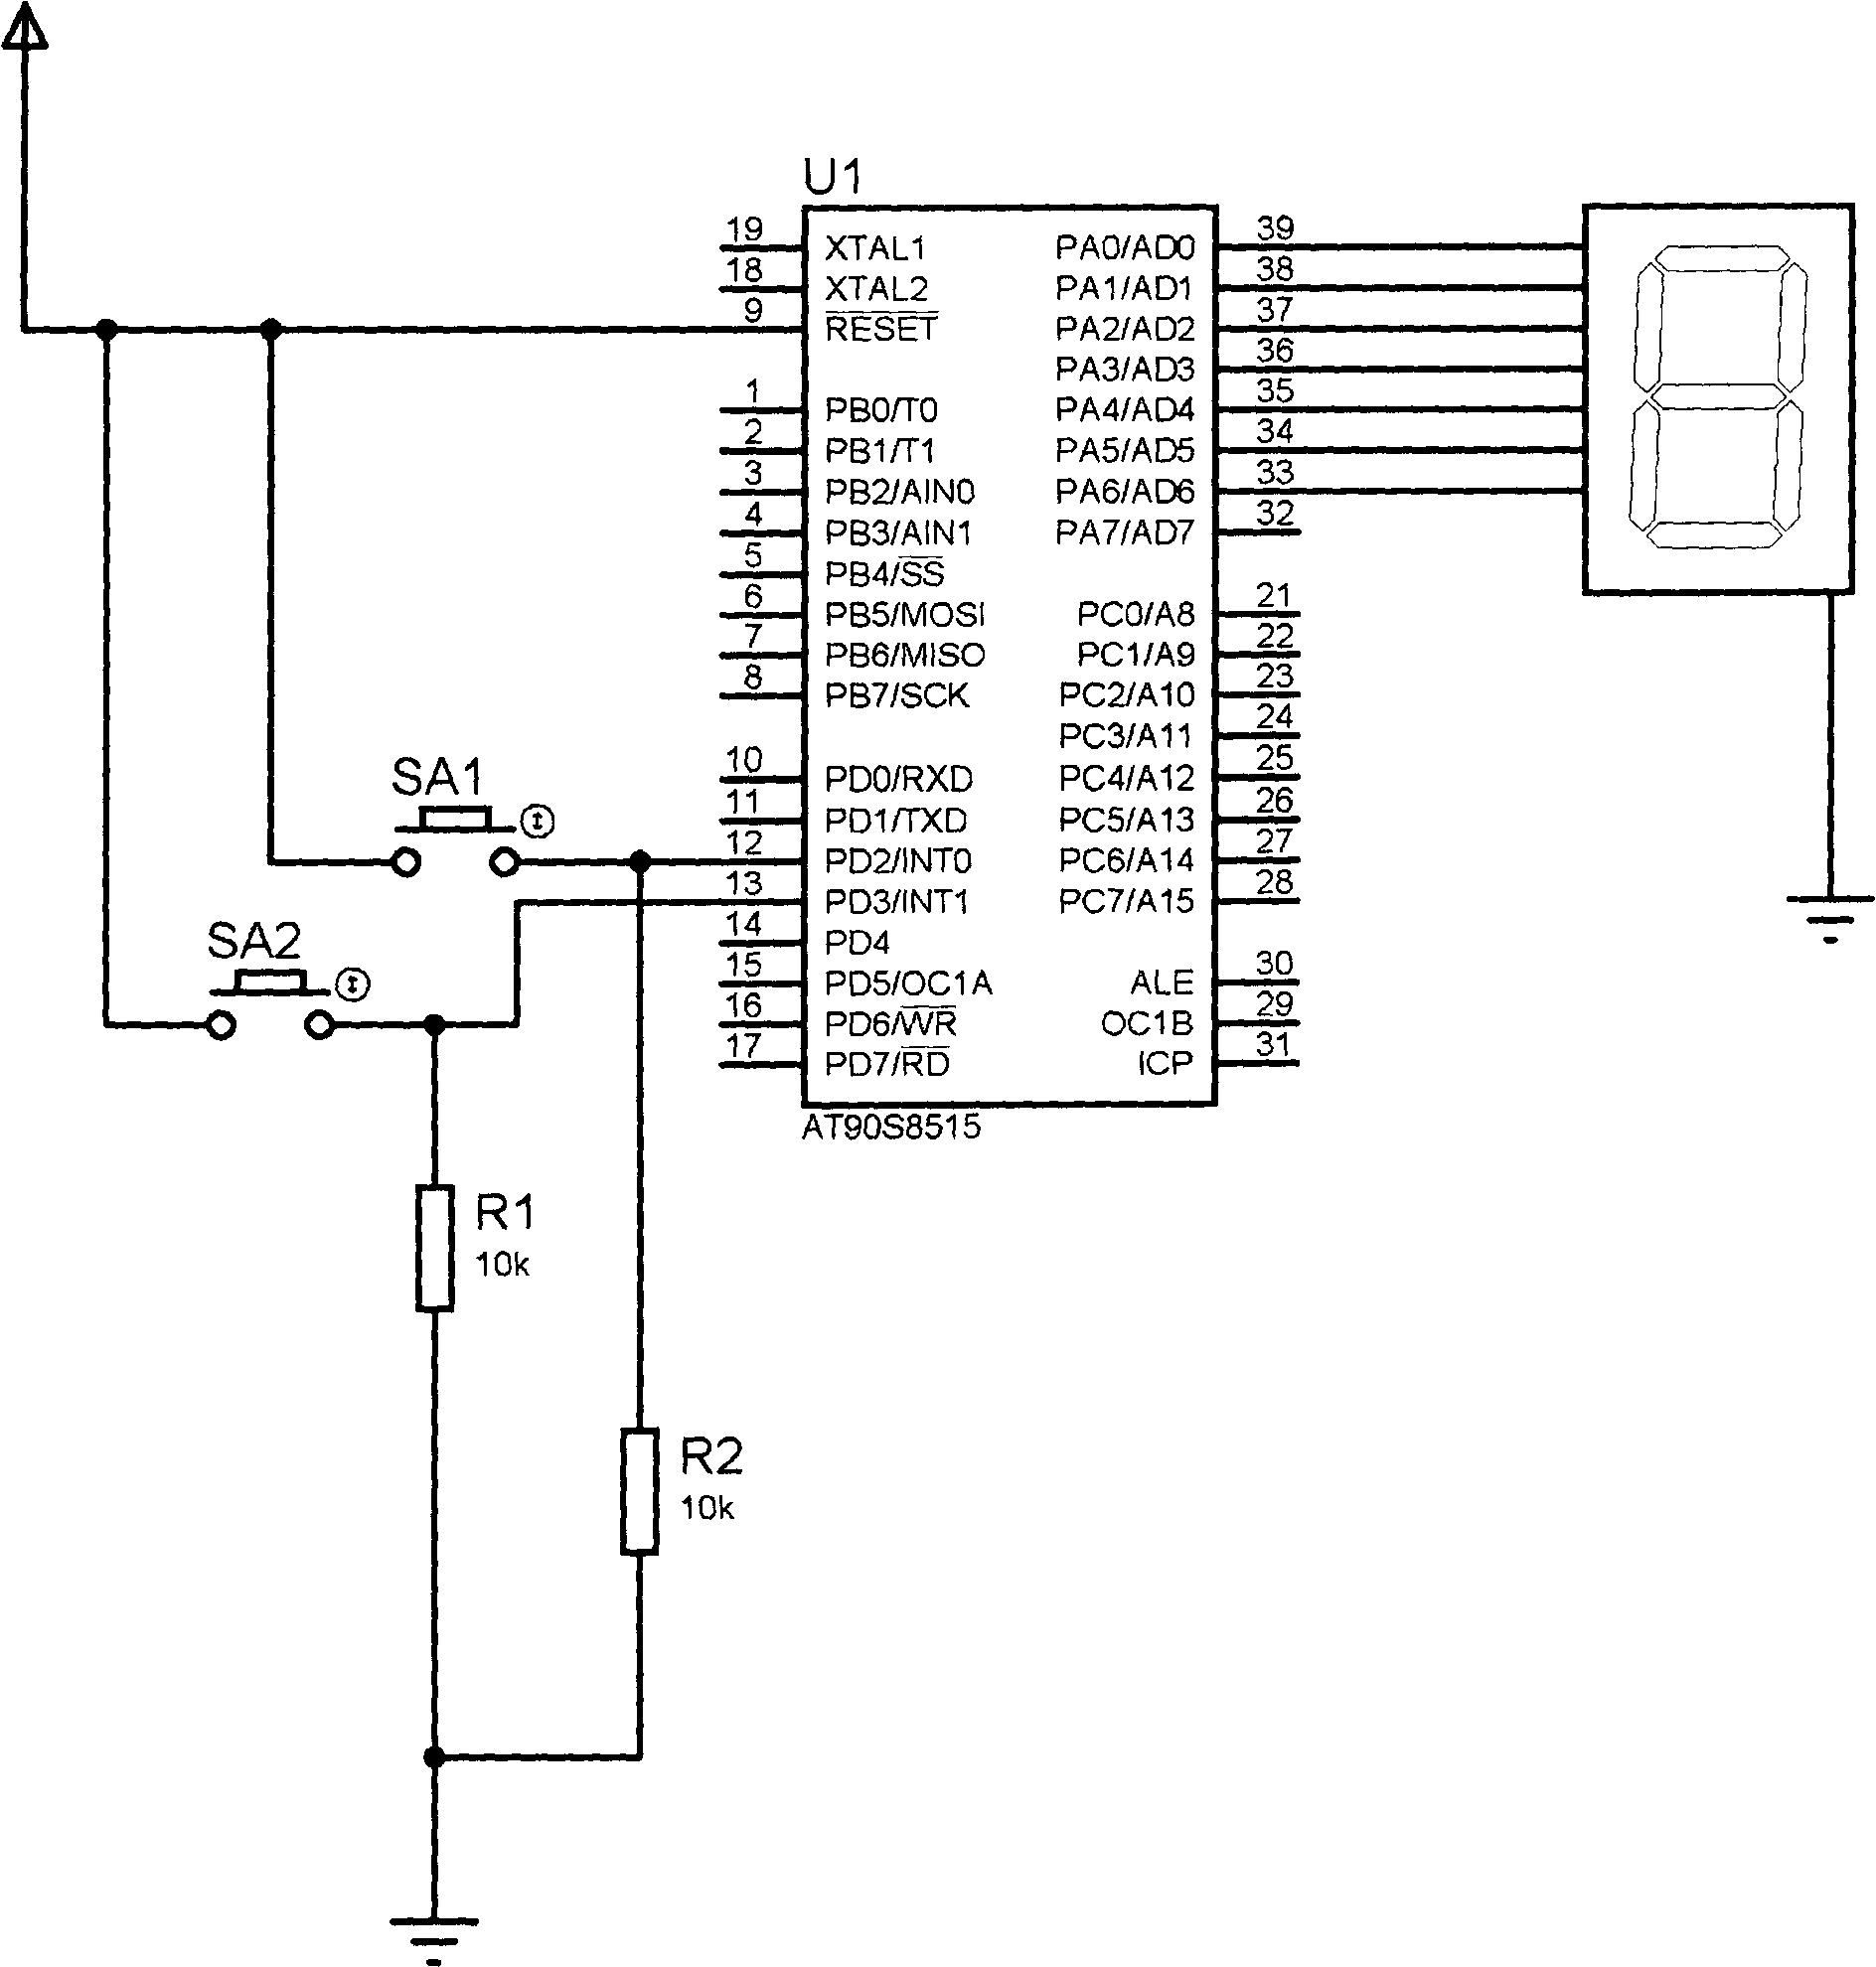
\includegraphics[scale=0.18]{images/example1.png}
\caption{Пример принципиальной электрической схемы.\\ На схеме должны быть обязательно подписаны используемые выводы микроконтроллера и номиналы резисторов и других элементов}
\label{fig:example1}
\end{figure}

\begin{figure}[b]
\centering
\includegraphics[scale=0.07]{images-gen/dia_example2.png}
\caption{Пример блок-схемы.\\ Осуществляется инициализация двух глобальных переменных, настройка порта ввода/вывода на вывод и настройка двух внешних прерываний. Обработчик внешнего прерывания 1 записывает флаг в глобальную переменную. Обработчик внешнего прерывания 0 проверяет флаг, если установлен, то ничего не делает. Иначе прибавляет к счётчику единицу, при достижении 10~--- обнуляет. И выводит цифру на индикатор}
\label{fig:example2}
\end{figure}

\end{document}
